% http://iproc.ru/interesting/hydro-history/1/
% http://iproc.ru/interesting/hydro-history/2/

\section{Краткая история гидродинамики}

\subsection{Определение понятия <<гидродинамика>>}

Что же такое гидродинамика? Энциклопедия дает следующее определение~\cite{wiki}:

<<Гидродинамика~--- раздел физики сплошных сред, изучающий движение идеальных и реальных жидкости и газа.
Как и в других разделах физики сплошных сред, прежде всего осуществляется переход от реальной среды, 
состоящей из большого числа отдельных атомов или молекул, к абстрактной сплошной среде, для которой и 
записываются уравнения движения.>>

Следует обратить внимание на то, что гидродинамика, несмотря на свое название («гидро»~--- вода, 
«динамика»~--- движение), изучает не только движение жидкости, но и движение газа, хотя на первый 
взгляд между ними очень много различий.

Помимо гидродинамики есть еще гидростатика, изучающая равновесие жидкостей. Но, в отличии от 
гидродинамики, законы гидростатики (законы Паскаля и Архимеда) просты и не подвергаются сомнению.

Несмотря на простоту законов, описывающих покоящуюся жидкость, движущаяся жидкость долгое время 
оставалась (и всё еще остается) неподвластна умам ученых. Многие ека философы пытались разгадать 
тайны течения воды (самой распространенной жидкости на Земле). Но зарождение гидродинамики как науки 
началось после открытия Ньютоном своих законов, которые стали отправной точкой для математического 
описания движения жидкости.

\subsection{Ранние попытки исследовать течение жидкости}

О том, как среда сопротивляется движению тела, можно узнать, наблюдая за падением тел в воде или в воздухе. 
Проведением подобных опытов одним из первых занялся Леонардо да Винчи (1452--1519). 
Его дело продолжил другой «шаробросатель»~--- Галилео Галилей (1564--1642). 
Сбрасывая с наклонной Пизанской башни тяжелые и легкие шары, он установил независимость 
скорости падения тяжелых тел от их веса и сформулировал один из величайших физических принципов~--- принцип инерции.

Бенедетто Кастелли (1577--1644) и Эванджелиста Торричелли (1608--1647)~--- двое из учеников 
Галилея,~--- попытались применить открытия своего учителя для объяснения течения воды.

В 1628 году Кастелли издал маленькую работу \textit{Della misura dell' acque correnti}, в которой он 
удовлетворительно для своего времени объяснил несколько явлений при движении жидкостей 
в реках и каналах; однако он допустил ошибку, предположив, что скорость вытекающей 
из сосуда воды пропорциональна глубине расположения отверстия под поверхностью воды в сосуде.

Торричелли заметил, что в фонтане, в котором вода вытекала из маленькой насадки, 
она поднималась до почти той же самой высоты, что и вода в бассейне, из которого она подавалась. 
На основе этого он предположил, что вода вытекает с той же скоростью, которую она получает 
при падении с высоты ее поверхности в сосуде (а падение предметов уже было изучено Галилеем). 
Он вывел теорему, согласно 
которой скорость вытекающей жидкости пропорциональна квадратному корню высоты воды в сосуде. 
Эта теорема была издана в 1643 году, в конце его трактата \textit{De motu gravium projectorum}, и была 
подтверждена экспериментами Рафаэлло Магиотти (1597--1656) на воде, вытекающей из различных 
насадок под различными давлениями (1648).

Теорема Торричелли использовалась многими последующими авторами, особенно 
Эдме Мариоттом (1620--1684), чей \textit{Traite du mouvement des eaux}, изданный после его смерти 
в 1686 году, основан на большом разнообразии тщательно проведанных экспериментов 
с движением жидкостей. В обсуждении некоторых из них он допустил ошибки, результаты 
других он рассматривал поверхностно. И он не сделал ни одного эксперимента для явного 
исследования уменьшения скорости вытекания воды в результате прохождения через тонкую трубку. 
Но он, кажется, первый, кто попытался объяснить несоответствие между теорией и экспериментом, 
заключающееся в уменьшении скорости воды, с помощью трения. Его современник Доменико 
Гульельмини (1655--1710), который был инспектором рек и каналов в Болонье, приписал 
это уменьшение скорости в реках к поперечным течениям, являющимся результатом неровностей дна. 
Но, поскольку Мариотт наблюдал подобные замедления движения даже в стеклянных трубах, 
где никакие поперечные течения не существовали, причина, назначенная Гульельмини, казалась 
Мариотту лишенной основания. Поэтому он расценил это замедление, как эффект трения. 
Он предположил, что нити воды, которые задевают стенки трубы, теряют часть своей скорости. 
Смежные нити, имеющие большую скорость, трутся о предыдущие и переносят уменьшение скорости 
далее к оси трубы. Нити затронуты подобным замедлением скорости пропорционально их 
расстоянию от оси трубы. Таким образом, средняя скорость потока становится меньше, и, 
следовательно, количество воды, вытекающей в единицу времени, из-за эффектов трения 
должно быть заметно меньше вычисляемого теоретически.

Эффекты трения и вязкости, как причины уменьшения скорости проточной воды, были 
замечены в труде \textit{Philosophiae Naturalis Principia Mathematica} сэра Исаака Ньютона 
(1643--1727), который пролил много света на несколько ветвей гидродинамики. 
В то время, когда декартовская теория вихрей преобладала, он нашел необходимым 
исследовать эту гипотезу. В ходе исследований Ньютон показал, что скорость 
любого слоя вихря~--- среднее арифметическое между скоростями слоев, которые 
прилегают к нему; из этого следовало, что скорость нити воды, перемещающейся в трубе, 
равна среднему арифметическому скоростей нитей, которые окружают ее. Используя в своих 
интересах эти результаты, Анри Пито (1695--1771) впоследствии показал, что замедление, 
являющееся результатом трения, обратно пропорционально диаметру труб, в которых 
перемещается жидкость.

Внимание Ньютона было также привлечено к исследованию вытекания воды из отверстия в основании 
сосуда. Он рассмотрел цилиндрический сосуд, полный воды, с маленьким отверстием в основании, 
из которого вытекала вода. Этот сосуд снабжался водой таким образом, что всегда оставался 
наполненным до одной и той же высоты. Он предположил, что цилиндрический столб воды разделен 
на две части. Первая, которую он назвал «потоком», является гиперболоидом вращения, который 
проходит через отверстие, а вторая~--- остаток воды в цилиндрическом сосуде. Он считал, что 
горизонтальные слои этого гиперболоида всегда в движении, в то время как остаток воды 
находится в состоянии покоя (своего рода поток внутри жидкости). В результате этой теории 
Ньютон получил, что скорость, с которой вода вытекает из отверстия, равна скорости, 
которую падающее тело получит, падая с половины высоты воды в бассейне. Это заключение, 
однако, абсолютно противоречило известному факту, согласно которому высота водной струи 
равна высоте бассейна, и Ньютон, кажется, знал об этом. Соответственно, во втором издании Начал, 
которое появилось в 1713 году, он пересмотрел свою теорию. Он обнаружил сужение струи, 
выходящей из отверстия, и нашел, что на расстоянии, приблизительно равном диаметру отверстия, 
сечение струи было меньше в два раза. Он расценил суженное сечение струи, как истинное отверстие, 
через которое вытекает вода из сосуда. В этом случае скорость истекающей воды как раз 
соответствует всей высоте воды в бассейне. Это означает, что его теория стала более 
соответствовать результатам опыта, хотя все еще сталкивалась с серьезными возражениями. 
Ньютон был также первым, кто исследовал движение волн.

\subsection{Парадигма Ньютона. Классическая механика}

Несмотря на неудачу Ньютона в исследовании движения жидкости, его законы (всемирного тяготения и три закона движения) 
совершили прорыв в математическом описании физических объектов. Становление механики и физики как точных наук началось с 
уравнения Ньютона («второй закон Ньютона»):
\begin{gather}
	m \frac{d \vec u}{d t} = \vec f
	\label{1}
\end{gather}
Здесь $m$~--- масса, $\vec u$~--- скорость, $t$~--- время, $\vec f$~--- сила.

Уравнение \ref{1} описывает изменение скорости материальной точки (или твердого тела) под действием силы.
 Его можно считать исходной парадигмой всей физики.

Уже через несколько лет после публикации Ньютоном своих Начал ученые заметили ту простоту (и ту точность получаемых 
результатов), с которой можно применять законы Ньютона для описания окружающего мира. Все попытки объяснить движение 
воды с этого момента делались на основе этих законов. Однако, применить их к жидкости оказалось совсем не простым делом.
 Пройдет еще 60 лет, прежде чем Эйлер сможет получить аналог второго закона Ньютона для жидкости.

В 1738 году Даниил Бернулли (1700--1782) издал свой труд \textit{Hydrodynamica seu de viribus et motibus fluidorum
commentarii}. Его теория движения жидкостей, основы которой были сначала изданы в его биографии под названием 
\textit{Theoria nova de motu aquarum per canales quocunque fluentes}, и сообщены в Академии Санкт-Петербурга 
еще в 1726 году, была основана на двух гипотезах, которые казались ему соответствующими опытным данным. 
Он предположил, что поверхность жидкости, содержащейся в сосуде и вытекающей из отверстия, остается всегда
горизонтальной. Жидкую массу он представил разделенной на бесконечное число горизонтальных слоев равного объёма,
касающихся друг друга. Скорость опускания слоёв обратно пропорциональна их ширине (горизонтальным сечениям сосуда).
Чтобы определить горизонтальное движение внутри каждого слоя, он использовал принцип \textit{ conservatio virium
vivarum}, и получил очень изящные решения. Но, в отсутствии общей демонстрации этих принципов, его результаты не
получили доверия.

Было желательно иметь более общую теорию, зависящую исключительно от фундаментальных законов механики Ньютона. 
Колин Маклорен (1698--1746) и Джон Бернулли (1667--1748, не путать с Даниилом Бернулли), которые придерживались 
этого мнения, решили проблему более прямыми методами. Первый~--- в его \textit{Fluxions}, изданных в 1742 году, 
а второй~--- в его \textit{Hydraulica nunc primum detecta, et demonstrata directe ex fundamentis pure mechanicis} 
(четвертый том его работ). Метод, используемый Маклореном, считался недостаточно строгим. Метод Джона Бернулли~--- 
тоже (по мнению Лагранжа, он страдал от недостатка четкости и точности).

Теория Даниила Бернулли также встретила сопротивление в лице Жана Лерона Даламбера (1717--1783), разработавшего 
свою теорию. Обобщая теорию маятников Якоба Бернулли (1654--1705, не путать с Джоном Бернулли и Даниилом Бернулли) 
он обнаружил принцип динамики, столь простой и общий, что он сводил законы движений тел к закону их равновесия. 
Даламбер применил этот принцип к движению жидкостей, дав образец его применения в конце его \textit{Dynamics} 
в 1743 году. Принцип был более полно развит им в \textit{Traite des fluides} (1744), в котором он дал простые 
и изящные решения проблем, касающихся равновесия и движения жидкостей. Он использовал те же гипотезы, что и 
Даниил Бернулли, хотя его исчисление было выстроено в совсем другой манере. Он рассматривал в каждый момент 
движение слоя жидкости, как составленное из движения, которое он имел в предыдущий момент, и движения, которое 
он потерял. Законы равновесия между потерями движения дали Бернулли уравнения, представляющие уравнения движения
жидкости. Оставалось желательным выразить уравнениями движение частицы жидкости в любом заданном направлении. 
Эти уравнения были найдены Даламбером из двух принципов: 1) прямоугольный канал, выделенный в массе жидкости, 
находящейся в равновесии, сам находится в равновесии, и 2) часть жидкости, переходящая из одного места в другое, 
сохраняет тот же самый объем, когда жидкость несжимаема, или изменяет объём, как будто она является упругой.
 Его остроумный метод, изданный в 1752 году в \textit{Essai sur la resistance des fluides}, был доведён до 
 совершенства в \textit{Opuscules mathematiques}, и был перенят Леонардом Эйлером (1707--1783).

\subsection{Парадигма Эйлера. Сплошная среда и модель сухой воды}

Решение вопросов движения жидкостей было произведено с помощью метода частных производных Эйлера. 
Это исчисление было впервые применено к движению воды Даламбером, и позволило ему и Эйлеру представить теорию
 жидкостей в формулировке, не ограниченной никакими особыми предположениями. Прежде чем перейти к этой теории, 
 нам понадобится понятие сплошной среды \cite{wiki}:

<<Сплошная среда — механическая система, обладающая бесконечным числом внутренних степеней свободы. Её движение 
в пространстве, в отличие от других механических систем, описывается не координатами и скоростями отдельных 
частиц, а скалярным полем плотности и векторным полем скоростей. В зависимости от задач, к этим полям могут 
добавляться поля других физических величин (концентрация, температура и др.) Если плотность сплошной среды 
постулируется равной константе, то такая сплошная среда называется несжимаемой. Однако с точки зрения 
математической строгости следует помнить об одной неточности: все реальные системы обладают пусть большим, 
но конечным числом степеней свободы (например, состоят из атомов). Сплошная же среда обладает не просто 
бесконечным, а несчетным числом степеней свободы.>>

Для применения уравнения Ньютона к движению сплошной среды следовало перейти к описанию течения в фиксированной 
точке пространства, то есть отнести массу и силу к единице объёма. Для этого же потребовалось ввести 
субстанциональное ускорение:
\begin{gather}
\frac{d \vec v}{d t} = \frac{\partial \vec v}{\partial t} + (\vec v, \nabla) \vec v
\label{2}
\end{gather}

Смысл этого выражения в том, что ускорение жидкости в фиксированной точке пространства равно сумме ускорения 
частиц жидкости и изменений скорости, приносимых течением из соседних областей. Жидкость течёт, и под 
действием своего течения переносит всё, что в ней находится, в том числе и скорость своего течения. Это 
трудно понять, но ещё труднее было к этому прийти.

Наконец, переход от отдельных тел к континууму потребовал вместо сосредоточенной в точке силы введения 
нормального напряжения~--- давления p. В отличие от ньютоновой механики оказалось, что напряжения не заданы 
априори, а самовозникают вследствие движения жидкости.

Эйлер выполнил переход к континууму. Выведенные им в 1755 году уравнения движения сплошной среды, не 
потерявшие актуальность и в наше время, так и называются — эйлеровыми:
\begin{gather}
\begin{cases}
\rho \frac{d \vec v}{d t} = - \nabla p \\
\nabla \vec v = 0
\end{cases}
\label{3}
\end{gather}
Здесь $\rho$~--- плотность жидкости. Эти уравнения описывают течение невязкой несжимаемой жидкости. 
Такую модель идеальной сплошной среды фон Нейман образно и остроумно назвал «моделью сухой воды». Она явилась
 первой парадигмой гидродинамики.

Первое уравнение представляет собой ни что иное, как закон Ньютона, выписанный для «кусочка жидкости». $\rho$ 
представляет собой массу этого кусочка, $ d \vec{v} / dt$~--- его ускорение. В правой части стоит сила, 
вызываемая давлением (точнее~--- градиентом давления). Основное отличие от второго закона Ньютона здесь в том,
что уравнение описывает не только изменение скорости под действием силы (давления), но и изменение силы (давления)
под действием скорости: левая и правая части здесь равноправны. Второе уравнение говорит о постоянстве объёма
 «кусочка жидкости»: он может менять свою форму, но не может менять объём; жидкость несжимаема.

Как уже было сказано, модель «сухой воды» не учитывает вязкость и сжимаемость жидкости. Но основная преграда, 
препятствовавшая её применению для широкого круга прикладных задач,~--- отсутствие границ у жидкости. Подобно 
электромагнитному полю течение занимает всё пространство. Герман фон Гельмгольц (1821--1894), пытаясь применить 
эйлеровы уравнения ко всё той же задаче об истечении жидкости из сосуда, в 1858 году предложил принципиально новую 
схему~--- истечение с отходящими от краёв отверстия разрывами (границами вода--воздух). Его схема находилась в 
визуальном согласии с истечением воды из крана вплоть до момента турбулизации и капледробления струи.

Введя поверхности разрыва, Гельмгольц сделал решающий шаг в приближении модели идеальной жидкости к действительности. 
У него такой поверхностью была свободная граница, но впоследствии в качестве поверхностей разрывов в гидродинамике 
использовались вихревые пелены, контактные разрывы и даже так называемые сильные разрывы. Ввиду этого концепция 
кусочно--разрывного течения идеальной жидкости, выдвинутая Гельмгольцем, существенно расширяет модель Эйлера. 
Справедливости ради, следует напомнить, что о возможности существования разрывных решений впервые упомянул Ньютон 
в Началах, но его рассуждения были ошибочны.

В рамках этой парадигмы удалось разработать теорию волн на воде, как в линейном, так и в нелинейном приближениях 
(Стокер, Уизем, Лайтхилл). История открытия солитона С.~Pасселом, Н.~Крускалом и М.Д.~Забуски вошла во все 
учебники по нелинейной механике.

Другую ветвь развития эйлеровой модели составила динамика идеального (невязкого и нетеплопроводного) газа. 
Отличительная особенность этой теории~--- непостоянство плотности газа во времени и в пространстве. С учетом 
этого факта уравнения \ref{3} примут вид:
\begin{gather}
\begin{cases}
\frac{d (\rho \vec v)}{d t} = - \nabla p \\
\frac{\partial \rho }{\partial t} + \nabla (\rho \vec v) = 0
\end{cases}
\label{4}
\end{gather}

Поскольку число независимых переменных увеличилось на 1 (добавилась плотность), для замыкания системы уравнений 
Эйлера требуется ещё одно уравнение, в качестве которого обычно выступает уравнение состояния (обычно эмпирическое),
связывающее плотность, давление и другие характеристики газа. Например, уравнение Клапейрона--Менделеева:
\begin{gather}
p = \frac{\rho}{\mu}RT
\label{5}
\end{gather}
где $\mu$~--- молярная масса, T~--- температура, R~--- универсальная газовая постоянная.

История газовой механики изложена Я.Б.~Зельдовичем. Ударную волну открыл «на кончике пера» Б.~Риман в 1876 году. 
Однако гипотезу о существовании ударной волны задолго до него, в 1848 году, высказал Стокс, но отказался от 
нее под влиянием критики В.~Томсона и своего ученика лорда Рэлея.

\subsection{Динамика вязкой жидкости. Уравнения Навье--Стокса}

Одними из основных элементов течения жидкости являются вихри, возникающие вследствие нелинейности процессов 
движения. В динамике вихрей различимы~--- но не разделимы~--- три процесса: рождение, эволюция и диффузия.
 Модель идеальной жидкости (сухой воды) описывает эволюцию, иногда~--- рождение, но никогда~--- диффузию вихрей.

Если бы сухая вода существовала, то, налив в стакан, мы не смогли бы размешать её ложкой. Такую воду невозможно 
раскрутить: её слои не трутся друг о друга. При движении ложки вода будет расходиться впереди и смыкаться за ложкой. 
Даже вращающаяся перегородка, занимающая весь стакан от края до края, не создаст вращение, а лишь будет 
двигать воду из стороны в сторону. И наоборот: вихрь, однажды созданный в такой воде, будет существовать вечно. 
Его можно деформировать, разделить, но нельзя остановить.

Для понимания процессов рождения и диссипации вихрей, а также процессов взаимодействия (трения) жидкости 
со стенками сосуда, понадобилось перейти к более сложной модели~--- модели «мокрой воды», учитывающей 
влияние вязкости жидкости \cite{wiki}:

<<Вязкость~--- внутреннее трение, свойство текучих тел (жидкостей и газов) оказывать сопротивление 
перемещению одной их части относительно другой.>>

Если парадигма Эйлера строилась на спекулятивной основе, исходя из основных принципов и понятий механики, 
то для построения новой парадигмы потребовались некоторые априори неизвестные характеристики свойств 
рассматриваемой сплошной среды: в данном случае~--- вязкости, а в общем случае~--- теплопроводности, 
сжимаемости, второй вязкости и так далее.

В гидродинамике имеются три точных закона сохранения: массы, импульса и энергии. На основе этих законов 
(первых принципов физики) выводятся уравнения движения.

Остальные законы~--- приближенные, эмпирические. К ним относятся так называемые законы состояния, 
определяющие зависимость коэффициентов переноса от макроскопических параметров: законы Клапейрона, Фика, 
Ньютона, Дарси и другие. Эти законы состояния получаются в рамках кинетической теории при изучении 
структуры среды в масштабе, меньшем по порядку величины, чем гидродинамический масштаб. Говоря другими словами, 
осредняются происходящие в среде внутренние физико--химические процессы по малым (атомно--молекулярным) масштабам.

Впервые уравнения движения вязкой жидкости выписал французский учёный и инженер Анри Навье (1785--1836). 
Для этого потребовалось ввести тензор напряжений, то есть учесть не только нормальные силы (давление), но 
и касательные силы. В правую часть уравнения \ref{3} Навье ввёл дополнительный член, ответственный за 
проявление вязкости. Жидкость, напряжения в которой линейно пропорциональны деформации, называется ньютоновой, 
потому что впервые такая гипотеза была выдвинута Ньютоном \cite{betyaev}:

<<Сопротивление, происходящее от недостатка скользкости жидкости, при прочих равных условиях предполагается 
пропорциональным скорости, с которою частицы жидкости разъединяются друг с другом.>>

Сегодня мы знаем, как понимать его расплывчатое выражение «скорости, с которой…». Это~--- поперечный градиент 
скорости жидкости. Однако в конкретной задаче о круговом движении Ньютон выводит ошибочное условие для трения, 
на что спустя 158 лет после выхода его Начал указал Джордж Стокс (1819--1903).

Для ньютоновой жидкости уравнения сохранили векторную форму:
\begin{gather}
\begin{cases}
\frac{d \vec v}{d t} = - \frac{1}{\rho} \nabla p + \mu \nabla^2 \vec v \\
\nabla \vec v = 0
\end{cases}
\label{6}
\end{gather}
Здесь $\mu$~--- коэффициент кинематической вязкости.

Большой вклад в исследование этого уравнения внёс все тот же Стокс. Поэтому уравнения (6), а также их 
обобщения на случай движения жидкостей с другими свойствами называются уравнениями Навье--Стокса. Уравнения 
Эйлера~--- частный случай уравнений Навье--Стокса при $\mu=0$.

Для завершения математической модели течения вязкой жидкости недоставало граничных условий на поверхности 
контакта жидкости с твёрдым телом (для сухой воды это было просто: она скользила по всем поверхностям). 
Такой контакт (жидкость~--- твёрдое тело или газ~--- твёрдое тело) происходит в тонком пристеночном слое, 
где следует учитывать шероховатость и атомно--молекулярную структуру сред. Уже Д.~Бернулли в 1738 году 
осознавал, что жидкость не может скользить по поверхности твёрдого тела \cite{betyaev}:

<<Наблюдаются огромные различия, главным образом, в части прилипания воды к стенкам трубы; это прилипание 
заведомо может в некоторых случаях вызывать невероятные эффекты.>>

Француз Жирар в 1813 году считал, что вблизи контактной поверхности имеется весьма тонкий слой покоящейся 
относительно тела жидкости.

Вторая гипотеза принадлежала Навье. На основании тех же усложнённых молекулярных предположений, которые 
привели его к выводу уравнений движения вязкой жидкости, он установил, что на твёрдой поверхности имеет 
место проскальзывание жидкости, причём скорость проскальзывания $\vec{v}_0$ пропорциональна напряжению 
трения, то есть $\vec{v}_0=\lambda \cdot \partial \vec v / \partial \vec n$, где постоянная $\lambda$ 
имеет размерность длины, а дифференцирование проводится по направлению внешней нормали к твёрдой поверхности.

Наконец, третью гипотезу о прилипании жидкости к твёрдой поверхности первым, по-видимому, выдвинул Кулон в 
1800 году. В результате многочисленных опытов, а также анализа, проделанного Стоксом в 1851 году и 
Максвеллом в 1879 году, было установлено, что условие прилипания справедливо, если среда не разрежена. 
Входящая в условие Навье постоянная $\lambda$ по порядку величины равна длине свободного пробега молекул 
газа. Гидродинамика не рассматривает явления, происходящие на таких малых масштабах.

В полном виде уравнения Навье--Стокса оказались слишком сложными для решения, особенно в докомпьютерную эпоху.

Решительное продвижение вперёд сделал Людвиг Прандтль (1875--1953) в 1905 году, предложивший асимптотическую 
концепцию пограничного слоя. В соответствии с этой концепцией при малой вязкости область течения жидкости
 можно разделить на две части: внутреннюю область, в которой вязкостью можно пренебречь, и тонкую приграничную
  область (пограничный слой), в которой жидкость течёт параллельно границам, а скорость жидкости падает до 
  нуля по мере приближения к краю области. На дне пограничного слоя выполняется условие прилипания, а на его 
  внешней границе решение сращивается с невязким внутренним пределом. Кроме того, давление в пограничном 
  слое оказывается известным и равным давлению во внешнем потоке. Этот факт снижает на 1 число неизвестных 
  функций, а значит, и число уравнений. Сам Прандтль главную идею выразил такими словами \cite{betyaev}:

<<Поток разделяется на две части, взаимодействующие друг с другом; с одной стороны, мы имеем «свободный поток», 
который можно рассматривать как не имеющий трения, согласно теоремам Гельмгольца о вихрях, и, с другой стороны, 
пограничные слои около твёрдых стенок. Движение этих слоёв регулируется свободной жидкостью, но эти слои придают,
в свою очередь, свободной жидкости её основные свойства путём выделения вихревых поверхностей.>>

О наличии пристеночного пограничного слоя было известно задолго до Прандтля. Поэтому не Прандтль открыл 
пограничный слой. Но он сделал большее, показав, что понятие пограничного слоя~--- асимптотическое, что 
разложение в пограничном слое сращивается с внешним решением. Концепция Прандтля, существенно упрощающая 
модель вязкой жидкости, открыла путь к решению прикладных задач. Прандтль создал мощную научную школу: 
Ж.~Аккерет, А.~Бетц, А.~Буземан, М.~Мунк, В.~Толмин, И.И.~Никурадзе, Х.~Шлихтинг и другие.

\subsection{Непознанная турбулентность}

Однако вскоре выяснилось, что в подавляющем большинстве реальных случаев ламинарное течение слабовязкой жидкости 
становится неустойчивым и рано или поздно переходит в турбулентное:

Турбулентность [...]~--- явление, заключающееся в том, что при превышении некоторого критического числа 
Рейнольдса и/или Релея (в частном случае при превышении скорости потока при постоянной плотности и диаметре
трубы и/или температуры на внешней границе среды) самопроизвольно образуются многочисленные нелинейные 
фрактальные волны и обычные, линейные различных размеров, без наличия внешних, случайных, возмущающих 
среду сил и/или при их присутствии.

Общий критерий возникновения турбулентности установлен Осборном Рейнольдсом (1842--1912) в 1883 году. 
Он подкрашивал ламинарную струйку тока во входной части стеклянной трубки и следил, когда течение станет 
турбулентным, фиксируя при этом критическое значение безразмерного определяющего параметра, названного 
впоследствии в его честь числом Рейнольдса. В Манчестерском университете, где Рейнольдс проводил свои опыты, 
сохранилась его экспериментальная установка.

\begin{figure}[htp]
\centering
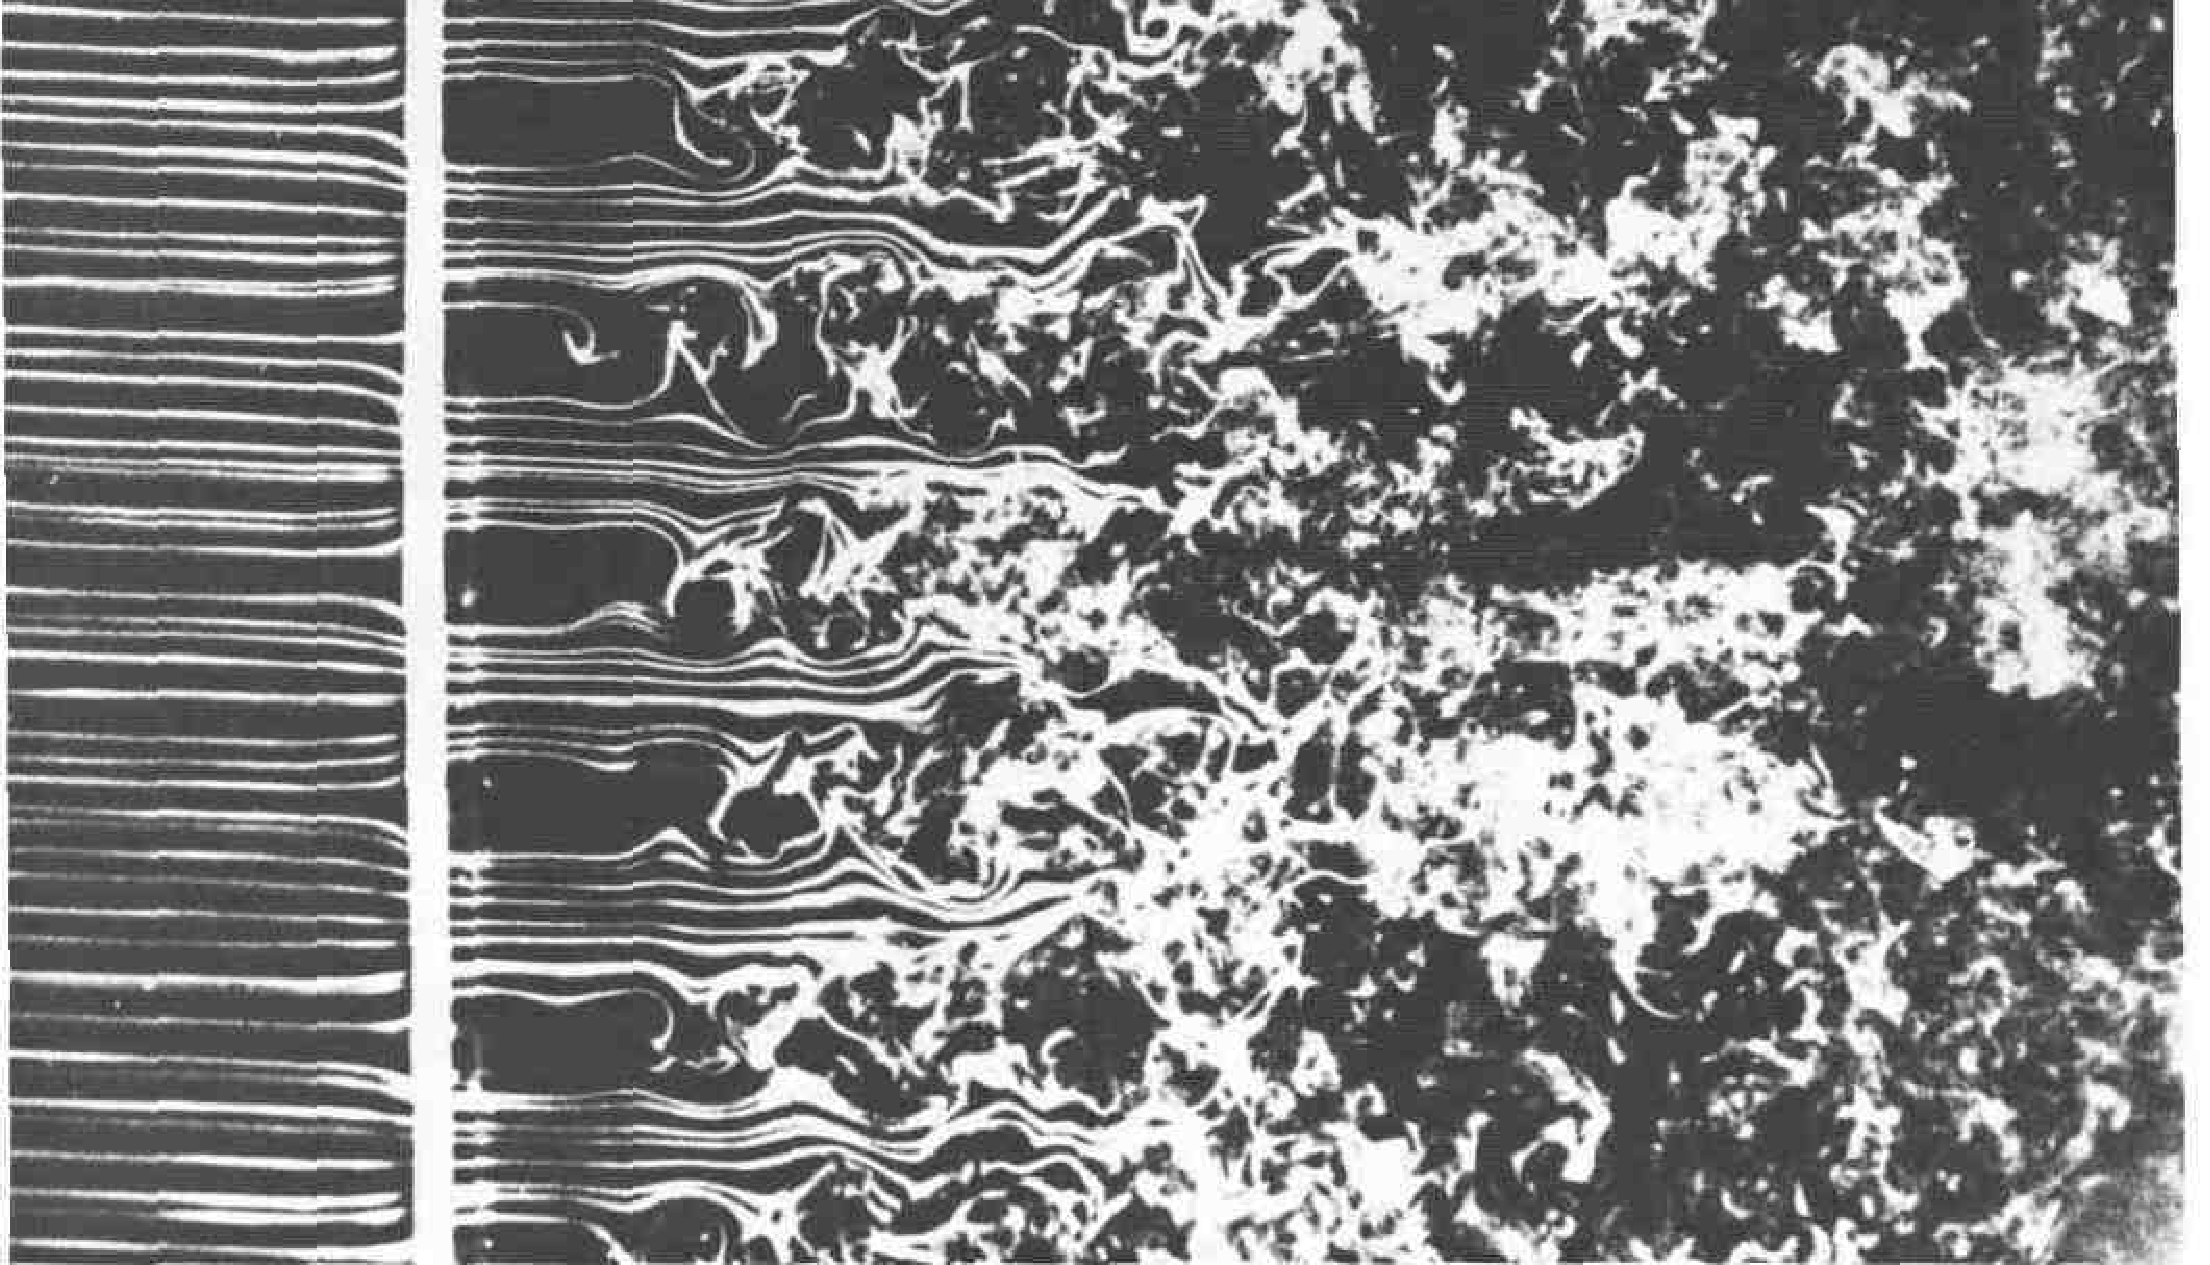
\includegraphics[width=0.7\linewidth]{historyImg/turb.pdf}
\caption{Порождение турбулентности решеткой. Изображние взято с сйта НИИ Мехяники МГУ.}
\label{img:turb}
\end{figure}

Представив скорость $u_i$ в виде суммы средней $\bar u_i$ и пульсационной $u_i'$ составляющих, а давление 
в виде $p=\bar p+p'$, Рейнольдс получил уравнения для средних величин, носящие его имя:
\begin{gather}
\rho\frac{\partial \bar u_j \bar u_i}{\partial x_j} = \frac{\partial}{\partial x_j}\left[ -\bar p \delta_{ij} +
\mu \left ( \frac{\partial \bar u_i}{\partial x_j} + \frac{\partial \bar u_j}{\partial x_i} \right) - 
\rho \overline{ u_i' u_j'} \right]
\label{7}
\end{gather}

Здесь подразумевается суммирование по индексу j. По сравнению с уравнением Навье--Стокса \ref{6} это 
уравнение включает дополнительные напряжения~--- так называемые напряжения Рейнольдса 
$\rho \overline{u_i^\prime u_j^\prime}$. Попытки найти их вид из первых принципов физики оказались безуспешными, 
поэтому уравнение \ref{7} стало базой для развития эмпирических теорий.

К недоопределенной системе \ref{7} следует добавить уравнения для пульсаций и правила осреднения. 
Полученную таким образом расширенную систему уравнений следует называть системой Рейнольдса. Решение 
этой системы кроме среднего и пульсационного слагаемого содержит еще волновой член.

Л.В.~Келлер и А.А.~Фридман дали аналитическую формулировку проблемы турбулентности, сведя задачу к 
бесконечной системе уравнений для статистических моментов. Джеффри Тейлор ввёл в рассмотрение корреляционные 
функции, а также впервые ввёл понятия об однородной и изотропной турбулентности.

Льюис Фри Ричардсон (1881--1953) высказал глубокие соображения о «каскадном процессе» передачи энергии 
по спектру от крупномасштабных мод к мелкомасштабным. Эта картина развитой турбулентности изображена 
Ричардсоном в стихотворении, которое входит во многие учебники по турбулентности:
\begin{center}
Big whorls have little whorls,

Which feed on their velocity;

Little whorls have smaller whorls,

And so on unto viscosity.
\end{center}

Ричардсон любил поэзию. Свою интуитивную теорию турбулентности он создал, вдохновлённый наблюдениями 
за эволюцией облаков.

Парадигма турбулентности ознаменовала превращение гидродинамики из чисто теоретической науки, 
из коллекции оригинальных, но оторванных от жизни решений, в прикладную науку. Разлившаяся река 
стремилась войти в берега актуальной полезности.

Наиболее важным вкладом в теорию турбулентности считаются 4 работы Андрея Николаевича Колмогорова 
(1903--1987), впервые опубликованные в 1941 году. В совокупности они так и называются~--- «теория К 41». 
Колмогоров занимался турбулентностью примерно полгода, до начала войны, а затем, в связи с требованиями 
военного времени, занялся баллистикой. Ещё 2 работы Колмогорова относятся к 1961--1962 годам и называются «теория К 62».

Были ли предшественники у Рейнольдса? Разумеется, каждый человек видел турбулентность в атмосфере, 
в ручье, в струе воды. Хаген ещё в 1839 году установил, что характер течения воды в трубе изменяется 
с увеличением напора. Он считал, что при определённых условиях в потоке возникают внутренние вихри, 
и это приводит к повышению сопротивления, и, следовательно, к уменьшению расхода воды.

Массивным блоком в основании теории турбулентности лежит теория вероятностей, прекрасные исторические 
обзоры которой даны Ширяевым (1998) и Гнеденко (2001). В теории турбулентности есть теория устойчивости 
и перехода ламинарного течения в турбулентное. Рэлею в 1880 году, В.~Орру и А.~Зоммерфельду в 1907--1908 
годах удалось линеаризовать задачу устойчивости в частном случае плоскопараллельного движения. Большое 
значение имеет теория устойчивости пограничного слоя и ламинарно--турбулентного перехода в пограничном слое 
(Бэтчелор, 2000). Следует упомянуть далеко продвинутую теорию изотропной турбулентности (Бэтчелор, 1955).

В XIX веке основной гидродинамической моделью являлась модель идеальной жидкости, в XIX--XX веках~--- 
модель вязкой жидкости. В XXI веке учёные стали вплотную заниматься построением физических и математических
 моделей турбулентности. Следует отметить, что парадигма турбулентности в гидродинамике еще не сформулирована,
  пока видны только её контуры... Построены математические модели случайных процессов в теории броуновского 
  движения и в квантовой механике. Однако построить адекватную модель истории человечества, макроэкономики 
  и турбулентности пока не удалось.

Невозможно провести чёткую границу между гидродинамикой и нелинейной механикой. И там, и там важна нелинейность. 
Актуально как изучение гидродинамических уравнений (Буссинеска, Кортевега--де Вриза и прочих), так и решение 
уравнений нелинейной механики (Шрёдингера, Гинзбурга--Ландау, Синус--Гордона и прочих), которые находят важные 
применения в гидродинамике.

Выдающийся физик Вернер Гейзенберг (1901--1976), серьёзно занимавшийся проблемой турбулентности, признался на 
смертном одре, что хотел бы задать Господу два вопроса~--- об основах теории относительности и о причине 
турбулентности. «Думаю, что Господь ответит мне на первый из них»,~--- галантно заключил он.

% \subsection*{Численное моделирование гидродинамических процессов}

%Усложнение математических моделей привело к тому, что человек перестал справляться с расчетами. Ответом на это  явилось создание компьютера. В то время казалось, что все задачи будут немедленно решены, что восторжествовал принцип пифагорейцев: «Всё есть число». Однако конец эмпирической эпохи в науке и технике не наступил, отодвинувшись на следующее столетие. Современный компьютер позволяет решать сложные задачи гидродинамики, физики плазмы, анализа загрязнения воздуха и грунтовых вод, создания новых лекарств, составления карт озонового слоя, сейсмического анализа. Численные расчёты востребованы как в фундаментальных науках, так и в прикладных.

% Для учёных и инженеров численный расчёт стал обыденным и мощным оружием наступления на непознанное. Численные расчёты практически вытеснили из употребления такие эмпирические методы, как приближения Бубнова--Галёркина в теории пограничного слоя, методы типа Бетца--Мультхопа в теории крыла большого удлинения, полуэмпирические методы в теории турбулентности и так далее. В настоящее время разработаны надёжные методы расчёта ламинарных течений, однако безэмпирический расчёт турбулентных течений пока ещё невозможен. Вычислительная гидродинамика~--- основная часть вычислительной математики, ибо в ней, как ни в одной области физики, задействована нелинейность и, как следствие, турбулентность.

\subsection{Несколько компьютерных иллюстраций численного моделирования течения жидкости}
\begin{figure}[htp]
\centering
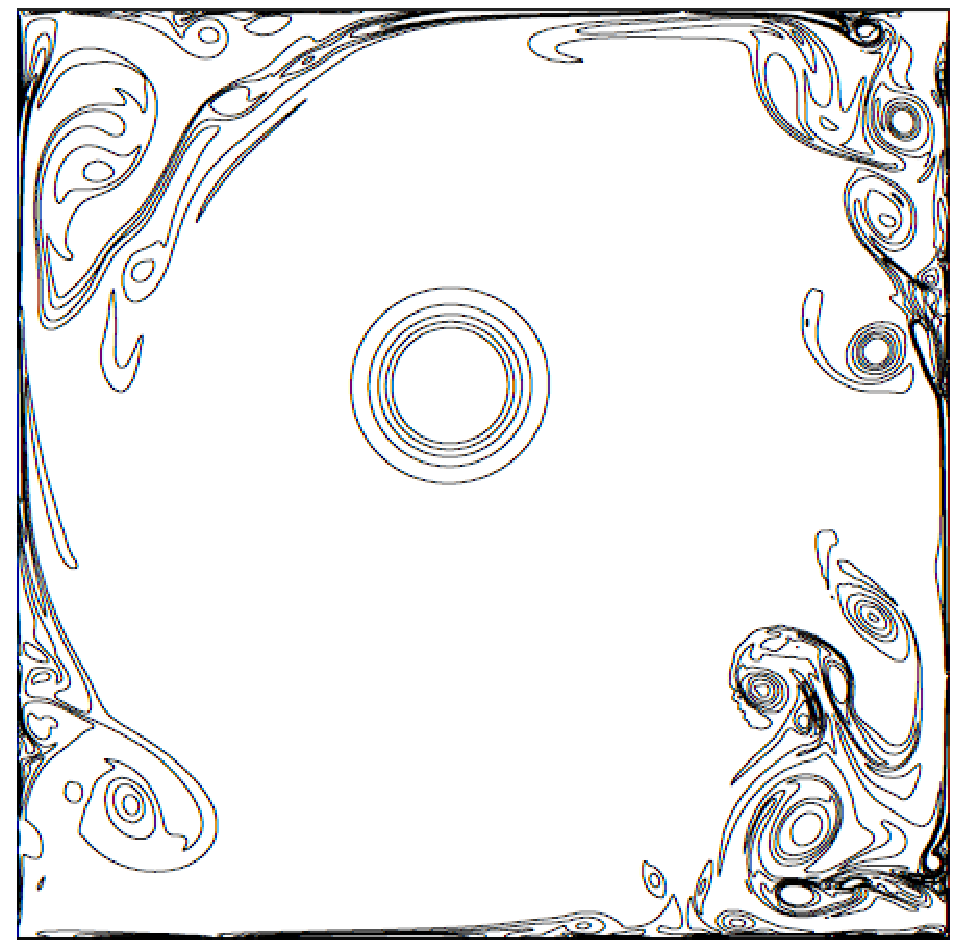
\includegraphics[width=0.5\linewidth]{historyImg/vortex_small.pdf}
\caption{Образование вихрей в вязкой жидкости возое границы из одного начального вихря, смещенного относиткльно центра облости. Покзаны изолини давления:  давление внутри вихря всегда ниже, чем давление снаружи}
\end{figure}

\begin{figure}[htp]
\centering
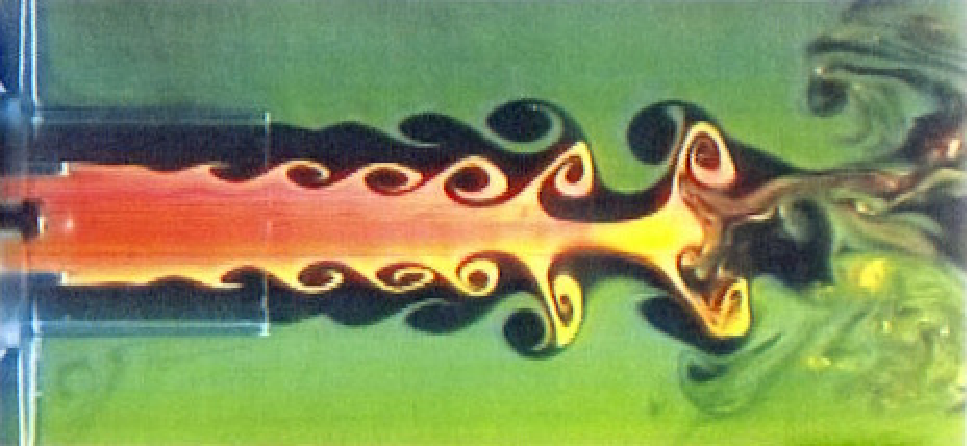
\includegraphics[width = 0.7\linewidth]{historyImg/jet_small.pdf}
\caption{Истечение жидкости из сопла}
\label{}
\end{figure}

\begin{figure}[htp]
\centering
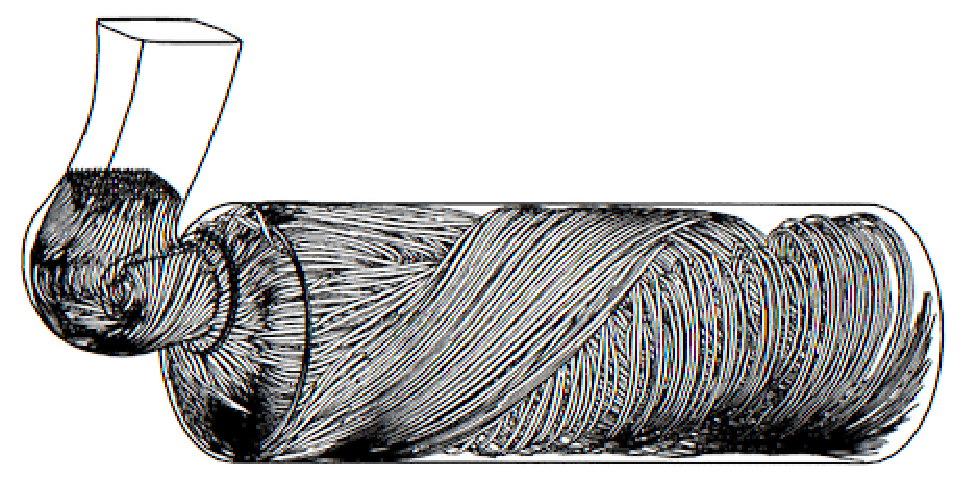
\includegraphics[width=0.7\linewidth]{historyImg/flow_small.pdf}
\caption{<<Нити тока>> жидкости, протекающей через трубу сложной формы}
\label{}
\end{figure}
\newpage

Материал опубликован на сатйте \cite{history}.
